\documentclass{article}
\usepackage[margin=0.5in]{geometry}
\usepackage{graphicx}

\title{Rutgers CS 440 Homework 1}
\author{Fulton Wilcox III, Dan Teytel, Long Tran}
\date{February 17 2023}

\begin{document}

\maketitle

    \begin{enumerate}
        \item[1.] \textbf{Understanding the Methods}
        \begin{enumerate}

            \begin{figure}[h!]
			\IfFileExists{diagram.png}{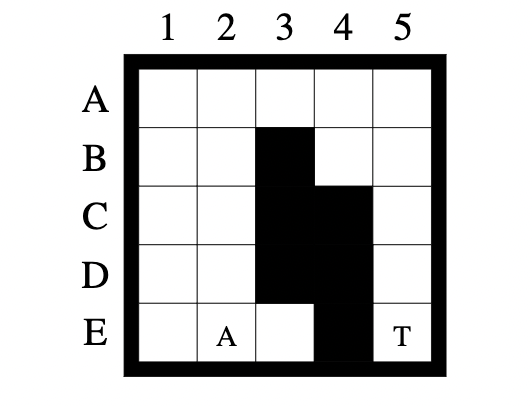
\includegraphics[width=0.2\textwidth]{diagram.png}}{No Figure Yet}
		\end{figure}
            
            \item[a.] In this example, the first move from A to the target will be to the right rather than up because the heuristic, which is the Manhattan distance from the current spot to the target, is 2 for the spot E3, while the heuristic for spot D2 is 4.  The step cost is 1 for both since this is the first step, so f(E3) $<$ F(D2).

            % \item[b.] Using A* search, the agent either reaches the target or discovers that it is impossible to reach the target.
            % To argue this, consider an agent and a target at any arbitrary spots on an arbitrarily generated maze.  An agent can expand its current node in any direction if that particular cell is unblocked and then move to the cell that has the lowest f(n).  Assuming the target is unreachable, as long as there is an unblocked cell adjacent to an expanded cell, A* will not terminate.  Therefore, in the worst case, A* will terminate only when there are no longer any adjacent un-expanded cells.  In the case when there is a path to the target, A* will terminate when every other path has greater cost than the cost to the target.

            % \item[1b.] In a finite gridworld, A* guarantees to find out the target or know it would be impossible to find it. The core concept of A* is greedy traversal search with optimized decisions of picking next moves to examine. Therefore, if there is no path leads to the target, A* will examine all cells in the gridworld and say it cannot reach the goal if they do not see it throughout the whole world.
            
            \item[1b] Let A represent an agent performing A* in a maze, M the total number of moves made by A, E be the number of expanded cells, and U the number of unblocked cells in the maze. 

            \item[Part 1] When A is using forward A*, each unblocked cell is only expanded once, and each move can only be made to a cell that has been expanded, meaning M $\le$ E $\le$ U $\le$ $U^2$, meaning M $\le$ $U^2$, proving M=O($U^2$) when A is performing forward A*.

            \item[Part 2] When A is using Adaptive A* or Repeated forward A*, A uses forward A* to generate a path through an unexplored maze, following that path until A reaches the goal or the path is blocked by a blocked cell. Let M(i) be the number of moves M in the "i"th iteration of A*. Since A stops when a blocked cell is in the path and does not enter any blocked cell or repeatedly enter an unblocked cell in the same iteration of A*, the statement M(i)$\le$ U still holds for the path proposed by A* for the unknown maze despite E $\le$ U not necessarily being true. Additionally, since A remembers the status of each cell adjacent to a visited cell and uses that status to generate a path with A*, and A* only stops on its path if the next cell in the path is blocked or the target, A will never stop at a given cell twice since A* would never create a path through a known blocked cell. 
            
            \item[] Suppose a worst case in which A needs to run A* after exploring each previously unexplored cell and A explores each unblocked cell before finding the target cell. This means A* is run by A a number of times equal to U. This means M can be defined by the equation M=M(i)*U. Since the statement  M(i)$\le$ U holds, the statement M= M(i)*U $\le$ U*U= $U^2$ is true, meaning M$\le$ $U^2$, or M=O($U^2$). 
            
            \item[4. ] Manhattan distances are consistent in this problem because it gives the shortest path estimation, in which there's no obstacles between start and goal.
            Let g(s, s') is the cost reach state s' from s. In 2D gridworld, Manhattan distances h(s) fits in the triangle inequality: 
            
            \[h(s) \leq g(s, s') + h(s'). \]
            
            Therefore, Manhattan distances are always the best cost to reach from start to goal out of all actions and states we can go.

            For adaptive heurictics, by updating the new h values: 
            $h_{new}(s) = g(s_{goal}) - g(s)$ \par

            $h_{new}(s)$ still satisfies admissibility by not overestimate the path costs.

            \textbf{Proving $h_{new}(s)$ is consistent:} \par
            Has shortest cost to goal $g(s_{goal})$ is shortest comparing with any combination of g(s') and heuristics h(s'). Comparing s' with another state s, subtract cost to reach s from start by both sides. We obtain that $h_{new}(s)$ is consistent.
            
            \[g(s_{goal}) \leq g(s') + h(s') \] 
            \[g(s_{goal}) - g(s) \leq g(s') - g(s) + h(s') \] 
            \[h_{new}(s) \leq g(s,s') + h(s') \leq g(s,s') + h_{new}(s') \]         

            By the above inequation, it is guaranteed that $h_{new}(s)$ is consistent either comparing with an s' state also has been expanded (s' state had its h-new(s')) or comparing with an s' state that has never been expanded.
                
            
        \end{enumerate}
    \end{enumerate}


\end{document}